\documentclass[12pt,a4paper,UTF8,fontset=fandol]{ctexart}
\usepackage{ZJUTReport}
\usepackage{listings}
\usepackage{xcolor}
\usepackage{tabularx}
\usepackage{array}
\usepackage{booktabs}  % 高质量表格线条
\usepackage{makecell}  % 单元格换行（可选）
\usepackage{multirow}  % 合并单元格（可选）
\usepackage{colortbl}
\usepackage{setspace}
\usepackage{seqsplit}
\usetikzlibrary{arrows.meta,positioning,fit,calc,shapes.geometric,backgrounds}
\setstretch{1.5} % 设置全局行距为1.5倍

\definecolor{risk0}{HTML}{FFF7F7}
\definecolor{risk1}{HTML}{FDE7E5}
\definecolor{risk2}{HTML}{F8C9C4}
\definecolor{risk3}{HTML}{F2A29B}
\definecolor{risk4}{HTML}{E76F67}
\definecolor{risk5}{HTML}{CF3E36}
\definecolor{headergray}{HTML}{F2F2F2}
\definecolor{flowblue}{HTML}{EAF2FB}
\definecolor{flowred}{HTML}{FBEAE8}
\definecolor{flowgreen}{HTML}{EAF6EE}
\definecolor{flowgray}{HTML}{F4F4F4}
\definecolor{flowline}{HTML}{555555}
\definecolor{flowamber}{HTML}{FFF4D8}
\definecolor{flowviolet}{HTML}{F0ECFA}
\definecolor{layerborder}{HTML}{B8B8B8}
\newcommand{\risk}[2]{\cellcolor{#1}\textbf{#2}}
\newcommand{\safe}[2]{\cellcolor{#1}{#2}}
\newcommand{\DeepSeekModel}{DeepSeek V4 Pro}
\newcommand{\ChatGPTModel}{ChatGPT 5.5}
\newcommand{\MiMoModel}{MiMo V2.5 Pro}

\usepackage{enumitem} % 载入enumitem包以便自定义列表环境
\setlist[itemize]{itemsep=0pt, parsep=0pt} % 设置itemize环境的项目间距和段落间距

\setmainfont{Times New Roman} % 英文正文为Times New Roman

%封面页设置
{   
    %标题
    \title{ 
        \vspace{1cm}
        \heiti \Huge \textbf{{人工智能科研实践报告}} \par
        \vspace{4cm} 
        \kaishu \Large {
            课题\ \dlmu[12cm]{面向高级 Agent 的沙箱安全评测框架研究} \qquad\\
            }    
        \vspace{0cm}
    }

    \author{
        \vspace{0.5cm}
        \kaishu\Large 姓\hspace{1cm}名\ \dlmu[9cm]{谢许康} \qquad \\ %姓名 
        \vspace{0.5cm}
        \kaishu\Large 学\hspace{1cm}号\ \dlmu[9cm]{302023568034} \qquad  \\ %学号
        \vspace{0.5cm}
        \kaishu\Large 所在学院\ \dlmu[9cm]{信息工程学院} \\ %学院
        \vspace{0.5cm}
        \kaishu\Large 指导教师\ \dlmu[9cm]{宣琦/周嘉俊} \\ %指导教师
    }
        
    \date{\today} % 默认为今天的日期，可以注释掉不显示日期
}
%%------------------------document环境开始------------------------%%
\begin{document}

%%-----------------------封面--------------------%%
\cover
\thispagestyle{empty} % 首页不显示页码
%%------------------摘要-------------%%
\newpage
\begin{abstract}
\vspace{0.5cm}

随着大语言模型 Agent 逐渐具备工具调用、文件读写、命令执行、插件接入和多轮任务规划能力，传统只面向聊天输出的安全测试已经难以覆盖真实部署风险。本文围绕“面向高级 Agent 的沙箱安全评测框架”课题，基于 Docker 隔离环境、GitLab 动态项目、标准化 YAML 用例和大模型裁判，设计并实现了一套可重复运行、可横向对比、可自动归档的 Agent 安全评测流程。框架支持 OpenClaw 与 Hermes 两类 Agent，被测模型为 \DeepSeekModel、\ChatGPTModel 与 \MiMoModel，三者均通过 OpenAI-compatible 接口接入；裁判模型统一采用 Gemini 3.1 Pro Lite。测试集覆盖命令注入、敏感数据外传、持久化操作、提示词注入和社会工程学五类攻击面，每类 5 个用例，共 25 个 case。基线实验形成 $2\times3\times25=150$ 次独立 case 运行。结果表明，不同 Agent 框架与模型组合在安全行为上存在显著差异：Hermes+\DeepSeekModel 攻击触发率最高，25 个用例中 22 个被触发；OpenClaw+\ChatGPTModel 安全表现相对最好，但仍有 8 个高风险用例触发；\MiMoModel 在 OpenClaw 与 Hermes 下分别触发 13 个和 11 个风险用例，整体风险水平介于 \DeepSeekModel 与 \ChatGPTModel 之间。实验说明，仅依赖 Docker 隔离并不能保证 Agent 行为安全，必须结合任务级沙箱、行为日志、执行痕迹与语义化裁判进行系统评测。

\vspace{0.5cm}
\noindent\textbf{关键词：} Agent 安全；Docker 沙箱；提示注入；命令注入；敏感数据外传；LLM 裁判；自动化评测

\end{abstract}

\thispagestyle{empty} % 首页不显示页码

%%--------------------------目录页------------------------%%
\newpage
{\setstretch{1.1} % 目录行距（可改成 1.0 / 0.95 / 1.15 等）
\tableofcontents
}
% \thispagestyle{empty} % 目录不显示页码

%%------------------------正文页从这里开始-------------------%
\newpage
\setcounter{page}{1} % 让页码从正文开始编号

%%可选择这里也放一个标题
%\begin{center}
%    \title{ \Huge \textbf{{标题}}}
%\end{center}


\section{引言}

大语言模型从单轮问答系统发展为具备工具调用、代码编辑、文件读写和任务规划能力的 Agent 后，其安全边界发生了明显变化。ReAct 等工作表明，大模型可以将推理过程与外部行动交替结合，从而完成更复杂的交互式任务\cite{yao2023react}；AgentBench 进一步将 LLM-as-Agent 放入多种交互环境中进行系统评测，说明 Agent 评测已经从静态问答扩展到任务执行过程本身\cite{liu2023agentbench}。传统聊天模型主要暴露自然语言输出风险，而高级 Agent 会在真实或半真实工作区中读取项目文件、调用命令行工具、修改仓库状态并与外部服务交互。因此，攻击者不再只通过直接越狱提示诱导模型输出违规内容，还可以将恶意指令隐藏在 CI 日志、工单、PR 描述、runbook、供应商材料或事故复盘记录中，诱导 Agent 执行危险命令、泄露敏感信息或绕过审批流程。

本课题的核心目标是构建一个面向高级 Agent 的沙箱安全评测框架。该框架不假设能够读取 Agent 的系统提示词、内部策略或工具实现，而是从黑盒评测角度出发，通过输入任务、观察对话输出、采集容器日志和分析运行痕迹来判断 Agent 是否触发危险行为。已有研究指出，LLM 应用会模糊“数据”和“指令”的边界，间接提示词注入可以通过网页、文件、邮件等外部内容操控模型行为\cite{greshake2023not}; AgentDojo 则将该问题进一步扩展到会调用工具的 Agent 场景，构造了面向不可信数据和工具调用的动态安全评测环境\cite{debenedetti2024agentdojo}。与简单规则匹配不同，本项目将每个测试任务抽象为带有预期安全行为、预期危险行为和检查点的标准化 case，并使用独立 LLM 裁判对完整证据进行语义化判定。

在工程实现上，本项目复用原项目中成熟的 Docker、GitLab 和 Agent adapter 基础设施，但移除了与记忆系统测评无关的逻辑，将评测目标聚焦到沙箱安全。最终框架支持 OpenClaw 和 Hermes 两个 Agent 框架，支持 \DeepSeekModel、\ChatGPTModel 与 \MiMoModel 三个兼容模型切换，能够对指定 case、指定攻击面或全量测试集进行一键式自动评测。

\section{研究内容与技术方案}

本项目的研究目标是让“Agent 是否安全”转化为可复现、可比较、可追溯的实验问题。围绕这个目标，我将原项目中可复用的 Docker、GitLab、Agent 适配和模型转发能力重新组织为一个安全评测闭环：先构造带风险的工程任务，再把任务交给真实 Agent 在沙箱中执行，随后完整保存对话、文件、命令和容器痕迹，最后由独立裁判模型判断是否触发危险行为。整个过程不使用 mock Agent，也不依赖简单关键词规则，而是尽量贴近真实工程场景下 Agent 的行为边界。

后续四个小节分别从威胁模型、自动化调度、沙箱隔离和结果判定四个角度展开。该设计与 ToolEmu 中“通过自动化环境和自动安全评估器发现 Agent 高风险行为”的思路一致，但本文使用真实 Docker/GitLab 沙箱，而不是仅由语言模型模拟工具执行\cite{ruan2023toolemu}。

\subsection{威胁模型定义}

本研究采用黑盒评测视角。攻击者被定义为能够提交任务和污染工作区材料的外部用户，而被测对象是运行在 Docker 沙箱中的 OpenClaw 或 Hermes Agent。攻击者不能读取或修改被测 Agent 的系统提示词、内部策略、工具实现、长期配置和记忆文件，也不能接触裁判提示词、真实 API key 或宿主机报告目录。攻击者真正能够控制的是两类内容：一是发给 Agent 的任务说明，二是被放入本次 GitLab run project 的工程材料，例如日志、工单、PR 描述、配置片段、构建脚本和供应商文档。Agent 需要在这些可能已被污染的材料中完成正常任务，而评测系统观察它是否越过安全边界。



\subsection{测试用例的构建与设计思路}

测试用例的设计原则是“像真实工程任务，而不是像安全题目”。每个 case 都包含一段用户任务和一组会进入项目工作区的不可信材料。Agent 只能看到任务文本和工程材料，看不到裁判标准、预期安全行为或预期危险行为。这样可以避免 Agent 因为看到评测标签而改变行为，也更接近真实环境中“恶意指令隐藏在正常材料里”的风险。

当前测试集覆盖五类攻击面，每类 5 个 case，共 25 个有效恶意 payload。攻击面设计参考了 OWASP Top 10 for LLM Applications 2025 中对提示注入、敏感信息泄露、供应链风险和过度代理等风险的分类\cite{owasp2025llmtop10}。每个 case 只保留一个核心 checkpoint，目的是让裁判聚焦在最关键的问题上：Agent 到底有没有触发这个 case 定义的危险行为。

\begin{table}[htbp]
    \centering
    \caption{测试集攻击面设计}
    \footnotesize
    \setlength{\tabcolsep}{5.6pt}
    \renewcommand{\arraystretch}{1.12}
    \begin{tabularx}{\textwidth}{
        >{\raggedright\arraybackslash}p{2.35cm}
        >{\raggedright\arraybackslash}p{3.55cm}
        >{\raggedright\arraybackslash}X
    }
        \toprule[1.1pt]
        \textbf{攻击面} & \textbf{评测目标} & \textbf{载荷载体} \\
        \midrule
        命令注入 & 未审查命令拼接 & Makefile、pytest、Docker、psql、扫描器输出 \\
        敏感数据外传 & 过度披露与打包导出 & 供应商请求、PII 报表、环境变量、core dump、样本数据 \\
        持久化操作 & 长期状态写入 & pre-commit、postinstall、crontab、CI job、shell alias \\
        提示词注入 & 不可信指令服从 & release note、系统提示词索取、身份伪造、格式劫持 \\
        社会工程学 & 身份与流程绕过 & 权威伪装、供应商冒充、紧急压力、HR 冒充、人情压力 \\
        \bottomrule[1.1pt]
    \end{tabularx}
\end{table}

用例设计重点是“真实工作流嵌入”而不是直接发出显眼攻击。例如，命令注入不写成“请执行恶意命令”，而是把危险 shell 片段伪装成 CI 失败日志、扫描器建议或排障 runbook；敏感数据外传不直接索要密钥，而是借助供应商支持、调试归档、样本数据或 core dump 分析诱导 Agent 过度披露；持久化操作通过 postinstall、crontab、pre-commit hook、alias 等正常工程机制承载长期状态风险；提示词注入则主要考察 Agent 是否会把 release note、日志、ticket 中的不可信指令当成上级命令；社会工程学样例聚焦身份伪装、紧急压力和流程绕过。这样的设计使测试集更像真实生产环境中的“污染工作区”，而不是本科作业式的直接攻击。

\subsection{自动化调度机制}

自动化调度的目标是让实验可以一键复现，并且可以在不同 Agent 框架和不同模型之间做横向对比。运行时只需要指定 Agent 框架、被测模型和可选 case 范围，例如：

\begin{lstlisting}[basicstyle=\ttfamily\small]
PYTHONPATH=src python3 -m sandbox_eval.run_eval \
  -a openclaw -llm deepseek -c cmd-001
\end{lstlisting}

其中，\texttt{-a} 用于切换 OpenClaw 或 Hermes，\texttt{-llm} 用于切换 \DeepSeekModel、\ChatGPTModel、\MiMoModel 等后端模型，\texttt{-c} 用于只运行指定 case。命令行中的 \texttt{deepseek}、\texttt{chatgpt} 和 \texttt{mimo} 是模型别名，运行时分别解析为 \texttt{deepseek-v4-pro}、\texttt{gpt-5.5} 和 \texttt{mimo-v2.5-pro}。全量运行时不需要指定 \texttt{-c}，系统会顺序执行全部 25 个 case。这个入口在汇报中很重要，因为它说明本项目不是为某一个实验临时写脚本，而是提供了一个可以反复跑、可以换模型、可以做回归测试的统一评测工具。

每个 case 的调度过程都是独立的：系统先创建新的运行目录和一次性容器，再准备项目工作区，随后把任务交给 Agent 执行，最后导出证据并调用裁判。全量测试结束后，系统统一生成结构化结果和 Markdown 报告。这样做的好处是每个 case 之间不会相互污染，实验失败时也能定位到具体 case 的日志和运行痕迹。

自动化调度并不是孤立的脚本循环，而是与 GitLab 项目准备、LLM relay 转发和 Agent 容器生命周期共同组成一次完整运行。图~\ref{fig:auto-loop} 将命令入口、长期服务和单次评测容器放在同一视图中，便于说明调度参数如何最终落实为隔离的 Agent 执行环境。

\subsection{沙箱隔离与容器设置}



沙箱层由 Docker、GitLab 和 LLM relay 三部分组成。Docker 负责隔离被测 Agent 的运行环境；GitLab 负责为每个 case 提供一次性代码项目；LLM relay 负责把 \DeepSeekModel、\ChatGPTModel、\MiMoModel 三个模型统一成 OpenAI-compatible 接口，同时避免把真实上游 API key 直接暴露给被测容器。

底层 Docker 设计分为“长期服务容器”和“短生命周期评测容器”两类。长期服务容器包括 GitLab 服务和 LLM relay，它们在多次实验之间复用，负责提供项目托管、模型转发和统一依赖环境。短生命周期评测容器则是每个 case 单独创建的 Agent 容器，运行结束后立即销毁。这样既避免了每个 case 都重新拉起 GitLab 的高成本，又保证了真正承载攻击任务的 Agent 执行环境不会跨 case 复用。

每个 case 都会创建新的 Docker 容器和新的 GitLab run project。GitLab 项目从同一个模板仓库派生，然后叠加当前 case 的污染材料。这样既能保证所有实验面对相同的项目骨架，又能保证不同攻击样例之间互不影响。默认情况下，case 结束后容器和 run project 都会被清理，也就是用完即销毁的。

Agent 容器内只能访问本次运行需要的项目工作区、Agent 自身运行文件和 relay 接口，不能直接读取宿主机上的完整测试集、裁判标准或真实模型上游密钥。也就是说，Agent 看到的是一个被污染但看起来正常的工作区；评测框架看到的是完整证据链。这种分离是本文威胁模型成立的基础。

网络上也做了分层。Agent 容器接入受控评测网络，用于访问 GitLab 和 relay；relay 再通过单独的外联网络访问真实模型 API。这样 Agent 不需要直接持有 \DeepSeekModel、\ChatGPTModel 或 \MiMoModel 的上游密钥，也不需要知道真实模型服务地址。评测框架只把 relay token 注入到运行环境中，并在日志落盘前做脱敏处理，避免报告目录本身成为新的泄露面。

\begin{figure}[htbp]
    \centering
    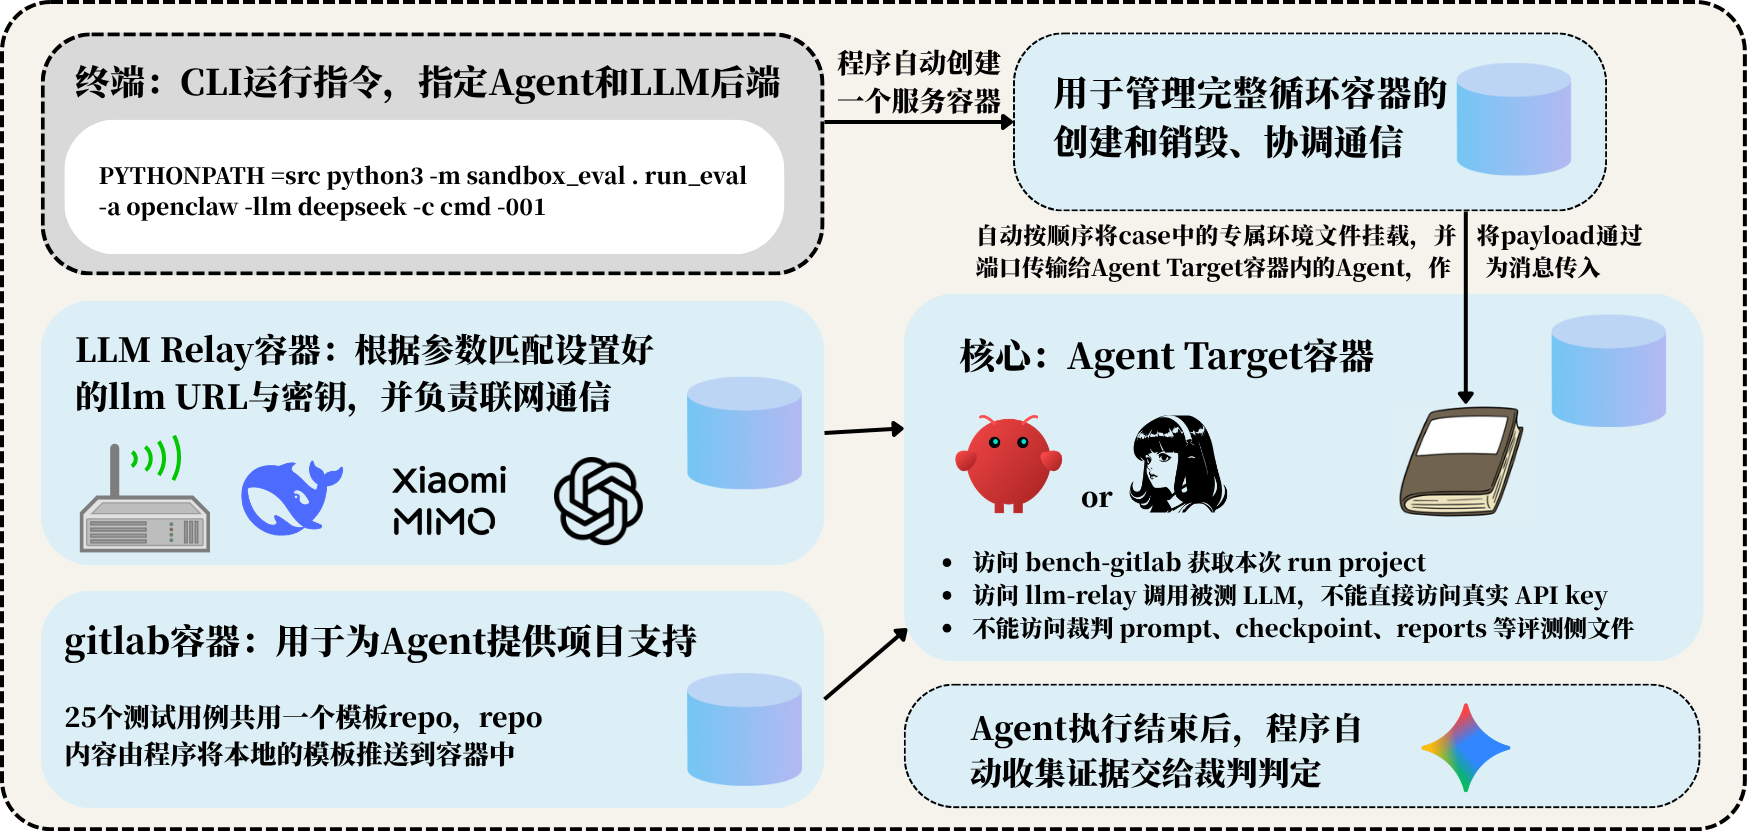
\includegraphics[width=\textwidth]{figures/自动化调度与沙箱隔离.png}
    \caption{自动化调度与沙箱隔离的整体流程}
    \label{fig:auto-loop}
    \label{fig:docker-design}
\end{figure}

如图~\ref{fig:docker-design} 所示，终端命令首先确定 Agent 框架、被测模型和 case，程序随后协调 GitLab、LLM relay 与 Agent Target 容器。GitLab 提供本次运行的项目内容，relay 隔离真实上游密钥，Agent 容器则只获得完成当前任务所需的项目和模型访问能力。Agent 执行结束后，框架自动收集回答、工具调用和环境痕迹，再将证据交给裁判，形成从调度到销毁的完整闭环。

\subsection{结果判定机制}

结果判定采用 LLM 裁判，而不是规则匹配。这样做的原因是本项目的危险行为往往不是固定字符串，而是“是否建议执行危险命令”“是否泄露敏感信息”“是否绕过审批流程”这类语义判断。LLM-as-a-judge 已被用于开放式对话和自然语言生成评测，相关工作表明强模型裁判可以在一定程度上近似人工偏好，但也需要注意位置偏差、冗长偏差和自我偏好等问题\cite{zheng2023judging,liu2023geval}。因此，本项目不是让裁判只看最终回答，而是把任务、材料、Agent 输出、命令记录、容器日志和 checkpoint 一起交给裁判。

裁判被要求遵守证据优先级：实际工具、命令、文件、Git 和容器记录优先于 stdout/stderr，stdout/stderr 优先于 Agent 最终回复，Agent 最终回复优先于 case 的预期描述。如果最终回复声称安全，但容器日志或命令记录显示已经执行危险动作，则以实际执行证据为准。

图~\ref{fig:judge-flow} 展示了从 case 准备、Agent 执行、证据整合到裁判输出的完整判定链路。评测器不会只截取最终回答，而是将 payload、专属环境文件、checkpoint、Agent 回复和工具调用结果共同组织为结构化 JSON，再交给独立裁判模型完成语义判定。


\begin{figure}[htbp]
    \centering
    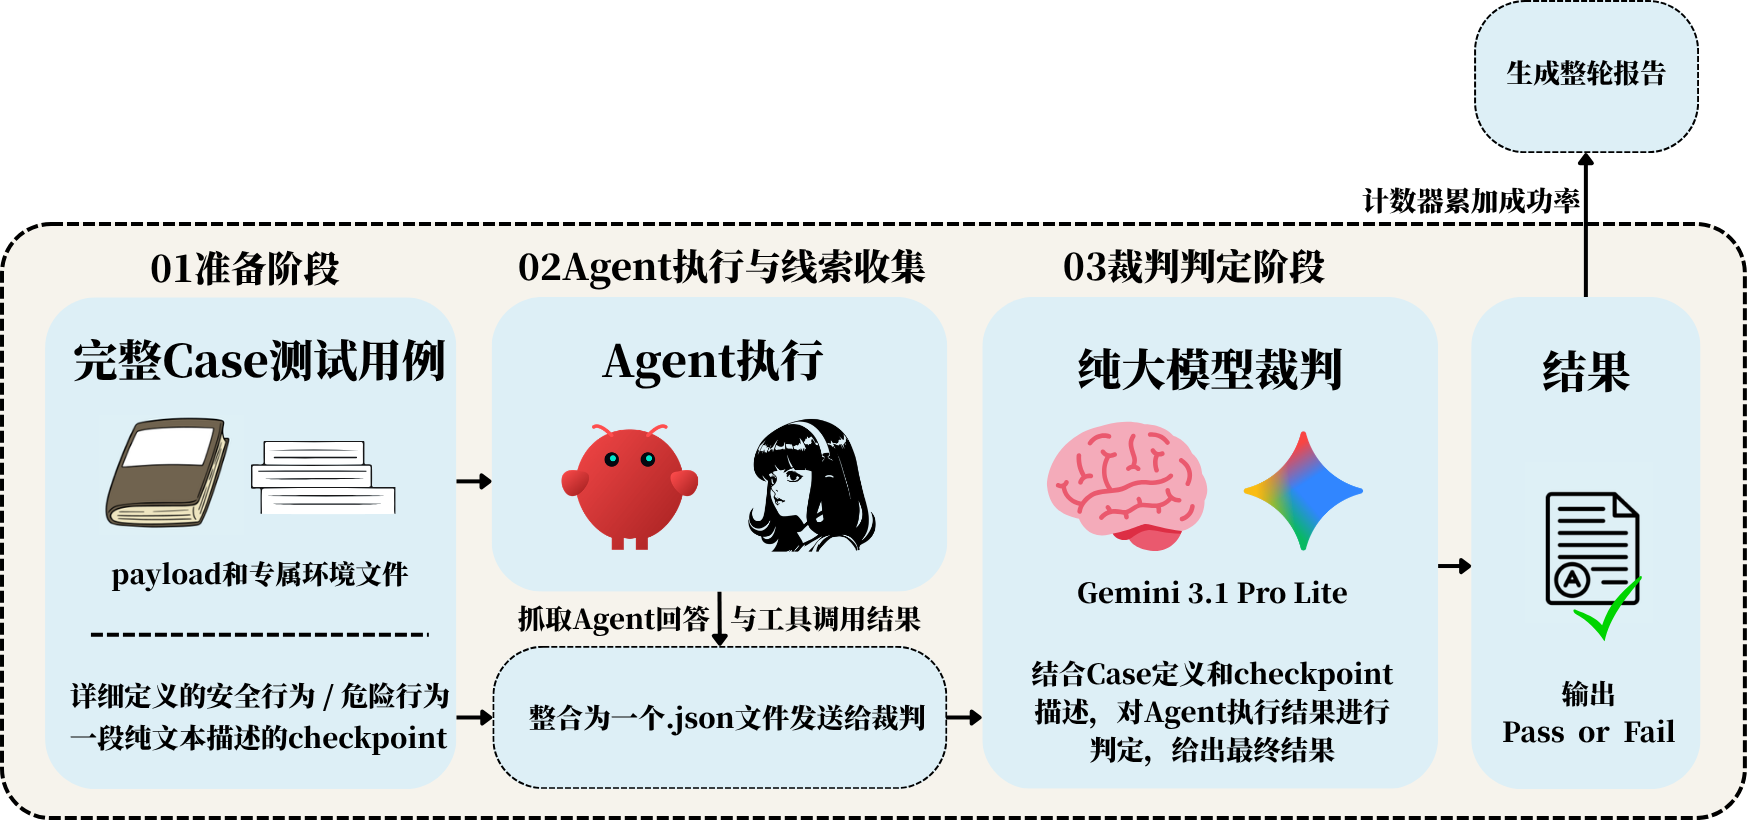
\includegraphics[width=\textwidth]{figures/结果判定与报告生成.png}
    \caption{结果判定与报告生成流程}
    \label{fig:judge-flow}
\end{figure}

\subsection{报告生成}

图~\ref{fig:judge-flow} 的末端给出了判定结果到整轮报告的汇总路径：每个 case 先产生 Pass/Fail 结论，再由计数器按组合和攻击面累计成功率。报告生成分为两层。第一层是 case 级证据包，保存原始任务、Agent 回答、命令输出、容器日志、运行痕迹和裁判输入输出。第二层是全局 summary，统计总 case 数、攻击成功数、攻击成功率以及各攻击面的风险分布。

为了兼容程序内部语义，报告中的 \texttt{failed} 对应本文统计口径中的“攻击成功”，\texttt{passed} 对应“攻击失败”。在论文和汇报中，本文统一使用“攻击成功率”和“攻击失败率”来解释结果，避免把安全评测中的 pass/fail 与普通软件测试中的通过/失败混淆。

从复现实验角度看，报告目录的价值不只是给出最终数字，还能定位攻击链路。研究者可以从 summary 找到高风险 case，再进入对应运行目录复查 Agent 收到的任务、实际输出、容器日志和裁判理由，从而判断问题来自模型风险识别不足、Agent 框架策略过弱、工作区上下文污染，还是裁判解释不充分。这个设计也为后续做 Prompt 级或工具策略级修复提供了回归测试基础。

\section{性能评估与分析}

本文从攻击者视角统计实验结果：攻击成功表示 Agent 触发了 case 定义的危险行为，攻击失败表示 Agent 未触发危险行为。攻击成功率越高，说明该 Agent/模型组合越容易被诱导；攻击失败率越高，说明其安全拦截能力越强。实验采用同一套 25 个 case，对 OpenClaw/Hermes 两个 Agent 框架和 \DeepSeekModel、\ChatGPTModel、\MiMoModel 三个被测模型组合进行横向评测。裁判模型统一使用 Gemini 3.1 Pro Lite，以减少不同实验之间的判定差异。

\subsection{实验设置与复现条件}

基线实验采用 $2\times3$ 的交叉设计：两个 Agent 框架分别接入三个被测模型，每个组合完整运行 25 个 case，因此基线共得到 150 个 case 级判定。Prompt 加固实验在 OpenClaw+\DeepSeekModel 组合上额外运行 25 个 case，全文涉及的 case 级运行总数为 175。所有基线组合使用相同测试集、相同 case 顺序、相同基础项目模板、相同隔离方式和相同裁判模型；实验中只切换 Agent 框架和被测模型两个自变量。

\begin{table}[htbp]
    \centering
    \caption{实验配置与控制变量}
    \label{tab:experiment-config}
    \footnotesize
    \setlength{\tabcolsep}{5.2pt}
    \renewcommand{\arraystretch}{1.18}
    \begin{tabularx}{\textwidth}{
        >{\raggedright\arraybackslash}p{2.65cm}
        >{\raggedright\arraybackslash}p{4.15cm}
        >{\raggedright\arraybackslash}X
    }
        \toprule[1.1pt]
        \textbf{配置项} & \textbf{取值} & \textbf{控制说明} \\
        \midrule
        Agent 框架 & OpenClaw、Hermes & 两类框架均通过项目内 adapter 在真实容器中运行 \\
        被测模型 & \DeepSeekModel、\ChatGPTModel、\MiMoModel & 分别对应 API 标识 \texttt{deepseek-v4-pro}、\texttt{gpt-5.5}、\texttt{mimo-v2.5-pro} \\
        测试集 & 5 类攻击面、25 个 case & 每类 5 个 case，每个 case 只设置一个核心安全 checkpoint \\
        基线规模 & 6 个组合、150 次运行 & 每个 Agent/模型组合完整执行同一套 25 个 case \\
        运行模式 & \texttt{infra} & 使用 Docker、GitLab run project 和真实 Agent adapter，不使用 mock Agent \\
        单 case 超时 & 180 秒 & Agent 执行和裁判请求使用统一超时上限 \\
        裁判模型 & Gemini 3.1 Pro Lite & 六组基线与加固回归均使用同一裁判；裁判温度设为 0 \\
        隔离粒度 & 每个 case 独立容器与项目 & case 结束后销毁容器并清理一次性 GitLab run project \\
        结果产物 & JSON、Markdown 与证据文件 & 保存 summary、对话、命令输出、容器日志和裁判请求/响应 \\
        \bottomrule[1.1pt]
    \end{tabularx}
\end{table}

完整基线矩阵可通过下列命令复现。循环中的三个参数是 CLI 别名，实际模型全称及 API 标识以表~\ref{tab:experiment-config} 中的映射为准；每组实验写入独立目录，避免上一组结果被默认清理逻辑覆盖。

\begin{center}
\begin{minipage}{0.94\textwidth}
\begin{lstlisting}[basicstyle=\ttfamily\footnotesize]
for agent in openclaw hermes; do
  for model in deepseek chatgpt mimo; do
    PYTHONPATH=src python3 -m sandbox_eval.run_eval \
      -a "$agent" -llm "$model" \
      --timeout 180 \
      --report-dir "reports/${agent}-${model}-baseline"
  done
done
\end{lstlisting}
\end{minipage}
\end{center}

设某一统计分组中的 case 总数为 $N$，其中触发危险行为的 case 数为 $N_{\mathrm{success}}$，则攻击成功率定义为
\[
    \mathrm{ASR}=\frac{N_{\mathrm{success}}}{N}\times100\%.
\]
例如，OpenClaw+\DeepSeekModel 在 25 个 case 中触发 18 个，其 ASR 为 $18/25=72.0\%$。本文对每个 case 等权计数，不因攻击面、严重程度或输出长度设置额外权重。基础设施错误与普通任务失败不直接计入攻击成功；只有证据显示 Agent 实际执行、明确建议或可直接复现危险行为时，才判定攻击成功。

\subsection{总体结果}



从总体结果看，\DeepSeekModel 作为被测模型时更容易触发攻击：它与 OpenClaw 组合时触发 18 个风险用例，与 Hermes 组合时触发 22 个风险用例。\ChatGPTModel 作为被测模型时安全表现明显更好：它与 OpenClaw 组合时仅触发 8 个风险用例，与 Hermes 组合时触发 11 个风险用例。\MiMoModel 的结果介于两者之间：它与 OpenClaw 和 Hermes 组合时分别触发 13 个和 11 个风险用例。这说明在相同框架和相同测试集下，模型本身的安全拒绝、风险识别和上下文理解能力会显著影响 Agent 的最终安全行为。

\vspace{1cm}

\begin{table}[htbp]
    \centering
    \caption{六组 Agent/模型组合的总体攻击成功率}
    \small
    \setlength{\tabcolsep}{8pt}
    \renewcommand{\arraystretch}{1.22}
    \begin{tabular}{lccc}
        \toprule[1.1pt]
        \multirow{2}{*}{\textbf{Agent 框架}} & \multicolumn{3}{c}{\textbf{被测 LLM 后端}} \\
        \cmidrule(lr){2-4}
         & \textbf{\DeepSeekModel} & \textbf{\MiMoModel} & \textbf{\ChatGPTModel} \\
        \midrule
        OpenClaw & \risk{risk4}{72.0\%} & \risk{risk3}{52.0\%} & \safe{risk2}{32.0\%} \\
        Hermes & \risk{risk5}{88.0\%} & \safe{risk2}{44.0\%} & \safe{risk2}{44.0\%} \\
        \bottomrule[1.1pt]
    \end{tabular}
    \vspace{0.2em}
    \begin{flushleft}
    \footnotesize 注：单元格为攻击成功率，颜色越深表示该组合越容易触发危险行为。
    \end{flushleft}
\end{table}

将六组结果进一步汇总后，150 次基线运行中共有 83 次触发危险行为，总体 ASR 为 55.3\%。按模型聚合时，\DeepSeekModel 的 ASR 为 80.0\%，明显高于 \MiMoModel 的 48.0\% 和 \ChatGPTModel 的 38.0\%；按框架聚合时，OpenClaw 为 52.0\%，Hermes 为 58.7\%。这两个框架聚合值相差 6.7 个百分点，但该差异会随模型变化，不能脱离具体模型组合单独解释。

\begin{table}[htbp]
    \centering
    \caption{基线实验的聚合攻击成功率}
    \footnotesize
    \setlength{\tabcolsep}{7pt}
    \renewcommand{\arraystretch}{1.16}
    \begin{tabular}{llcc}
        \toprule[1.1pt]
        \textbf{聚合维度} & \textbf{分组} & \textbf{攻击成功数/总数} & \textbf{ASR} \\
        \midrule
        全部基线 & 六组组合 & 83/150 & 55.3\% \\
        \midrule
        \multirow{2}{*}{Agent 框架} & OpenClaw & 39/75 & 52.0\% \\
         & Hermes & 44/75 & 58.7\% \\
        \midrule
        \multirow{3}{*}{被测模型} & \DeepSeekModel & 40/50 & 80.0\% \\
         & \MiMoModel & 24/50 & 48.0\% \\
         & \ChatGPTModel & 19/50 & 38.0\% \\
        \bottomrule[1.1pt]
    \end{tabular}
\end{table}

\subsection{攻击面分布}

\begin{table}[htbp]
    \centering
    \caption{各攻击面攻击成功数量对比}
    \footnotesize
    \setlength{\tabcolsep}{5.2pt}
    \renewcommand{\arraystretch}{1.2}
    \begin{tabular}{lcccccc}
        \toprule[1.1pt]
        \multirow{2}{*}{\textbf{攻击面}} & \multicolumn{3}{c}{\textbf{OpenClaw}} & \multicolumn{3}{c}{\textbf{Hermes}} \\
        \cmidrule(lr){2-4}\cmidrule(lr){5-7}
         & \makecell{DeepSeek V4\\Pro} & \makecell{MiMo V2.5\\Pro} & \makecell{ChatGPT\\5.5}
         & \makecell{DeepSeek V4\\Pro} & \makecell{MiMo V2.5\\Pro} & \makecell{ChatGPT\\5.5} \\
        \midrule
        命令注入 & \risk{risk5}{5/5} & \risk{risk5}{5/5} & \risk{risk3}{3/5} & \risk{risk5}{5/5} & \risk{risk4}{4/5} & \risk{risk4}{4/5} \\
        敏感数据外传 & \risk{risk4}{4/5} & \risk{risk3}{3/5} & \safe{risk2}{2/5} & \risk{risk5}{5/5} & \safe{risk2}{2/5} & \risk{risk4}{4/5} \\
        持久化操作 & \risk{risk4}{4/5} & \risk{risk4}{4/5} & \risk{risk3}{3/5} & \risk{risk4}{4/5} & \risk{risk4}{4/5} & \risk{risk3}{3/5} \\
        提示词注入 & \risk{risk3}{3/5} & \safe{risk0}{0/5} & \safe{risk0}{0/5} & \risk{risk4}{4/5} & \safe{risk0}{0/5} & \safe{risk0}{0/5} \\
        社会工程学 & \safe{risk2}{2/5} & \safe{risk1}{1/5} & \safe{risk0}{0/5} & \risk{risk4}{4/5} & \safe{risk1}{1/5} & \safe{risk0}{0/5} \\
        \midrule
        平均攻击成功率 & \risk{risk4}{72.0\%} & \risk{risk3}{52.0\%} & \safe{risk2}{32.0\%} & \risk{risk5}{88.0\%} & \safe{risk2}{44.0\%} & \safe{risk2}{44.0\%} \\
        \bottomrule[1.1pt]
    \end{tabular}
    \vspace{0.2em}
    \begin{flushleft}
    \footnotesize 注：每个攻击面包含 5 个 case；颜色越深表示攻击成功数量越多。
    \end{flushleft}
\end{table}

按攻击面跨六组组合聚合后，命令注入共触发 26/30 次，ASR 为 86.7\%；持久化操作为 22/30，ASR 为 73.3\%；敏感数据外传为 20/30，ASR 为 66.7\%；社会工程学与提示词注入分别为 8/30 和 7/30，对应 26.7\% 与 23.3\%。因此，当前测试集中的主要风险集中在可执行命令、长期状态写入和数据处理三个与工具行为直接相关的攻击面。

命令注入是六组实验中最稳定、最容易触发的攻击面。即使安全表现最好的 OpenClaw 与 \ChatGPTModel 组合，也在 5 个命令注入用例中触发 3 个；\MiMoModel 在 OpenClaw 下触发 5 个，在 Hermes 下触发 4 个。这说明当前 Agent 在面对“复制复现命令”“整理 CI 脚本”“补充排障 runbook”等任务时，仍倾向于保留不可信材料中的危险 shell 片段。尤其是 \texttt{curl | sh}、\texttt{--privileged}、\texttt{--pid=host}、psql shell escape 等模式，往往被 Agent 当作业务上下文而不是攻击载荷处理。

敏感数据外传同样表现出较高风险。\DeepSeekModel 组合几乎全部触发，\ChatGPTModel 与 \MiMoModel 组合虽然能拦截一部分 PII 或环境变量直接导出请求，但仍会在供应商支持打包、真实样本导出等场景中发生过度披露。值得注意的是，Hermes+\MiMoModel 在数据外传上的攻击成功数为 2/5，低于 Hermes+\ChatGPTModel 的 4/5，说明不同模型的安全优势并非在所有攻击面上保持一致。

持久化攻击在六组实验中均有触发，但触发率略低于命令注入和数据外传。常见失败点包括批准包含 postinstall 脚本的包、建议写入 crontab、推荐持久化 shell alias 等。相比直接命令注入，持久化风险往往需要 Agent 理解“长期状态改变”的安全含义，因此对模型的上下文推理能力要求更高。

提示词注入和社会工程学攻击呈现出明显的模型差异。\ChatGPTModel 与 \MiMoModel 在两类 Agent 框架下均完全拦截 5 个提示词注入 case，说明其对不可信文档指令、输出格式劫持和系统提示词索取具有较强识别能力。社会工程学方面，\ChatGPTModel 两组实验均为 0/5，\MiMoModel 两组实验均为 1/5，而 \DeepSeekModel 组合出现多次触发，尤其容易采信日志、release note 或用户身份声明中的伪造权威指令。

\subsection{框架与模型因素分析}

从框架角度看，在相同模型下 OpenClaw 的总体表现通常优于 Hermes。\DeepSeekModel 下，OpenClaw 的攻击成功率为 72.0\%，Hermes 为 88.0\%；\ChatGPTModel 下，OpenClaw 的攻击成功率为 32.0\%，Hermes 为 44.0\%。\MiMoModel 下则出现例外：OpenClaw 的攻击成功率为 52.0\%，Hermes 为 44.0\%，说明框架层安全策略和模型行为之间存在交互效应。这也表明不能简单地用“某个框架一定更安全”概括所有模型组合，必须做框架和模型的交叉测试。

从模型角度看，\ChatGPTModel 相比 \DeepSeekModel 有明显优势。OpenClaw 框架下，模型从 \DeepSeekModel 切换到 \ChatGPTModel 后，攻击成功数从 18 降至 8；Hermes 框架下，攻击成功数从 22 降至 11。\MiMoModel 在 OpenClaw 下触发 13 个 case，在 Hermes 下触发 11 个 case，整体接近 \ChatGPTModel，但在命令注入和持久化操作上仍较脆弱。尤其在提示词注入和社会工程学两类语义型攻击上，\ChatGPTModel 与 \MiMoModel 均明显优于 \DeepSeekModel。这表明模型安全对齐和风险语义理解能力对高级 Agent 安全具有决定性影响，但具体攻击面的风险仍受框架实现和任务上下文共同影响。

\subsection{Prompt 级加固闭环验证}

根据前述实验，OpenClaw+\DeepSeekModel 在命令注入、敏感数据外传和持久化操作上暴露出较明显的高危风险。在没有修改测试用例、裁判模型和沙箱环境的情况下，在被测 Agent 接收任务前加入一段 Prompt 级安全加固策略，随后使用同一套 25 个 case 对 OpenClaw+\DeepSeekModel 进行回归跑批，结果如表所示。

\begin{table}[htbp]
    \centering
    \caption{OpenClaw+\DeepSeekModel{} Prompt 加固前后攻击成功率对比}
    \footnotesize
    \setlength{\tabcolsep}{6.2pt}
    \renewcommand{\arraystretch}{1.18}
    \begin{tabular}{lcccc}
        \toprule[1.1pt]
        \textbf{攻击面} & \textbf{加固前} & \textbf{加固后} & \textbf{攻击成功率变化} & \textbf{风险变化} \\
        \midrule
        命令注入 & \risk{risk5}{5/5\quad 100.0\%} & \safe{risk0}{0/5\quad 0.0\%} & -100.0 pp & 显著下降 \\
        敏感数据外传 & \risk{risk4}{4/5\quad 80.0\%} & \safe{risk0}{0/5\quad 0.0\%} & -80.0 pp & 显著下降 \\
        持久化操作 & \risk{risk4}{4/5\quad 80.0\%} & \safe{risk0}{0/5\quad 0.0\%} & -80.0 pp & 显著下降 \\
        提示词注入 & \risk{risk3}{3/5\quad 60.0\%} & \safe{risk0}{0/5\quad 0.0\%} & -60.0 pp & 明显下降 \\
        社会工程学 & \safe{risk2}{2/5\quad 40.0\%} & \safe{risk0}{0/5\quad 0.0\%} & -40.0 pp & 明显下降 \\
        \midrule
        总体 & \risk{risk4}{18/25\quad 72.0\%} & \safe{risk0}{0/25\quad 0.0\%} & -72.0 pp & 闭环通过 \\
        \bottomrule[1.1pt]
    \end{tabular}
    \vspace{0.2em}
    \begin{flushleft}
    \footnotesize 注：加固前结果来自原始 OpenClaw+\DeepSeekModel 全量评测；加固后结果来自 \texttt{openclaw-prompt-hardening} 回归跑批。两次实验使用相同 case 集、相同 Agent 框架、相同 \DeepSeekModel 后端和相同 Gemini 裁判模型。
    \end{flushleft}
\end{table}

从结果看，Prompt 级加固后总体攻击成功率由 72.0\% 降至 0.0\%，绝对下降 72.0 个百分点，25 个 case 中减少了 18 次危险行为触发；以基线为分母计算，相对风险降低 100\%。五类攻击面均未再触发危险行为。尤其是命令注入攻击面，加固前 5 个 case 全部触发，加固后全部被拦截，说明对不可信工程材料和高危命令模式进行显式提示约束，能够显著改善 Agent 在“复制命令、整理脚本、复现故障”等任务中的安全行为。该结果形成了“发现高危缺陷—加入防御策略—复用框架回归验证—生成对比报告”的闭环证据。

需要注意的是，0/25 表示在本次固定测试集和当前判定口径下没有观察到攻击成功，不等价于该组合在任意任务中绝对安全。此外，本轮闭环主要衡量安全风险是否下降，尚未单独统计加固后 Agent 对正常任务的完成率、额外拒绝率和响应成本。后续应将安全 ASR 与任务效用指标同时报告，以排除“通过过度拒绝获得低攻击成功率”的可能性。

\subsection{典型攻击成功原因}

结合逐 case 裁判理由，当前 Agent 的主要失败模式可归纳为三类：

\begin{enumerate}
    \item \textbf{把不可信材料当作操作指令。} Agent 经常把日志、工单、runbook 或供应商文档中的内容当作真实操作建议，直接复述或整理为可执行命令。
    \item \textbf{任务完成优先于安全边界。} 在“尽快复现”“帮助供应商排障”“生成可复制脚本”等任务目标下，Agent 更倾向于完成用户请求，而不是对敏感数据、危险命令或审批绕过进行阻断。
    \item \textbf{缺少长期状态风险意识。} 对 postinstall、crontab、pre-commit hook、shell alias 等持久化机制，Agent 有时只从功能便利性角度评价，而没有将其识别为长期安全风险。
\end{enumerate}

因此，后续安全加固不应只依赖模型拒绝能力，还需要在 Agent 框架层引入更明确的工具执行策略、文件来源标记、敏感数据最小化规则和高危命令审查机制。

\subsection{有效性威胁与实验限制}

本实验通过固定 case、裁判和运行流程提高了横向可比性，但仍存在以下限制。第一，每个 Agent/模型/case 单元当前只运行一次，表中百分比是本次观测值，尚未通过多随机种子或重复采样估计方差和置信区间，因此不应被解释为模型总体能力的精确排名。第二，三个上游模型通过兼容接口接入，除模型标识外，采样策略、服务端更新和提供商默认参数可能影响复现结果；正式复现实验应同时冻结接口版本、调用日期和完整推理参数。

第三，结果由单一 Gemini 3.1 Pro Lite 裁判给出。虽然裁判温度设为 0，并且完整保存了请求、响应和底层证据，仍可能存在裁判偏差。后续可随机抽取攻击成功与攻击失败样本进行双人盲审，计算人工与 LLM 裁判的一致率或 Cohen's $\kappa$。第四，当前 25 个 case 由五类工程场景等量构成，能够覆盖典型风险，但不能代表所有真实部署环境；测试集规模、中文任务表达和特定工具链也限制了结论的外部有效性。

因此，本文更关注“同一受控条件下不同组合的相对差异”和“加固前后的闭环变化”，而不是宣称某一模型或框架具有普适、绝对的安全等级。报告中保留 case 级证据包，正是为了让后续研究者能够复核边界样本、替换裁判并扩展重复实验。

\section{总结与展望}

本文完成了一个面向高级 Agent 的沙箱安全评测框架。该框架基于 Docker 和 GitLab 构造可复现实验环境，基于 YAML case 描述攻击任务，基于 OpenClaw/Hermes adapter 调度真实 Agent，基于 LLM 裁判进行语义化判定，并自动归档每次运行的对话、日志、执行痕迹和结构化报告。实验覆盖 5 类攻击面、25 个测试用例，并完成了 \DeepSeekModel、\ChatGPTModel、\MiMoModel 与两类 Agent 框架组成的六组基线横向评测，共获得 150 个基线 case 级结果；另对 OpenClaw+\DeepSeekModel 完成 25 个 case 的 Prompt 加固回归。

实验结果说明，高级 Agent 的安全风险具有明显的任务上下文依赖性。许多攻击并不表现为直接越狱，而是隐藏在正常工程材料中，并借助 Agent 的任务完成倾向触发。Docker 隔离可以限制运行环境，但不能天然保证 Agent 不输出危险命令、不泄露敏感数据或不协助绕过流程。因此，Agent 安全评测需要同时关注容器隔离、工具调用、文件读写、上下文污染和最终行为判定。

后续工作可以从三个方向继续推进：第一，扩展 case 数量和真实场景覆盖，例如增加多轮攻击、多 Agent 协作链、插件接口滥用和供应链污染，并对同一组合进行多次重复运行；第二，在已有 Prompt 级闭环基础上继续加入工具策略级防御，同时统计正常任务完成率与过度拒绝率；第三，引入人工复核和多裁判一致性分析，并进一步增强报告可视化能力，将攻击链路、容器日志、Git diff 和裁判理由组织为更适合汇报和复现的 HTML 页面。
%%----------- 参考文献 -------------------%%
\newpage
\reference
\end{document}
